\documentclass[border=14pt]{standalone}
\usepackage[T1]{fontenc}
\usepackage[scaled=1.0]{helvet}
\renewcommand{\familydefault}{\sfdefault}
\usepackage{amsmath}
\usepackage{sansmath}
\sansmath
\hyphenpenalty=10000
\exhyphenpenalty=10000
\usepackage{xcolor}
\usepackage{tikz}
\usetikzlibrary{arrows.meta,positioning,calc,fit,backgrounds}
\definecolor{cblue}{HTML}{CFE2F8}
\definecolor{cpeach}{HTML}{F9DDD2}
\definecolor{cmint}{HTML}{D3EFE1}
\definecolor{cgrey}{HTML}{ECEBE7}
\definecolor{cline}{HTML}{6B6B6B}
\definecolor{clabel}{HTML}{555555}
\tikzset{
  blk/.style={draw=cline, line width=1.1pt, rounded corners=6pt, align=center, inner sep=6pt, minimum height=2.1cm, text width=#1},
  blk/.default=5.0cm,
  data/.style={blk=#1, fill=cgrey}, data/.default=5.0cm,
  ctrl/.style={blk=#1, fill=cblue}, ctrl/.default=5.0cm,
  path/.style={blk=#1, fill=cpeach}, path/.default=5.0cm,
  ana/.style={blk=#1, fill=cmint}, ana/.default=5.0cm,
  wire/.style={-{Stealth[length=9pt,width=7pt]}, draw=cline, line width=1.1pt},
  dwire/.style={wire, dashed},
  lab/.style={font=\normalsize, text=clabel},
  lane/.style={font=\large\bfseries, text=clabel},
}
\newcommand{\nt}[2]{{\LARGE #1}\\[3pt]{\Large #2}}

\begin{document}
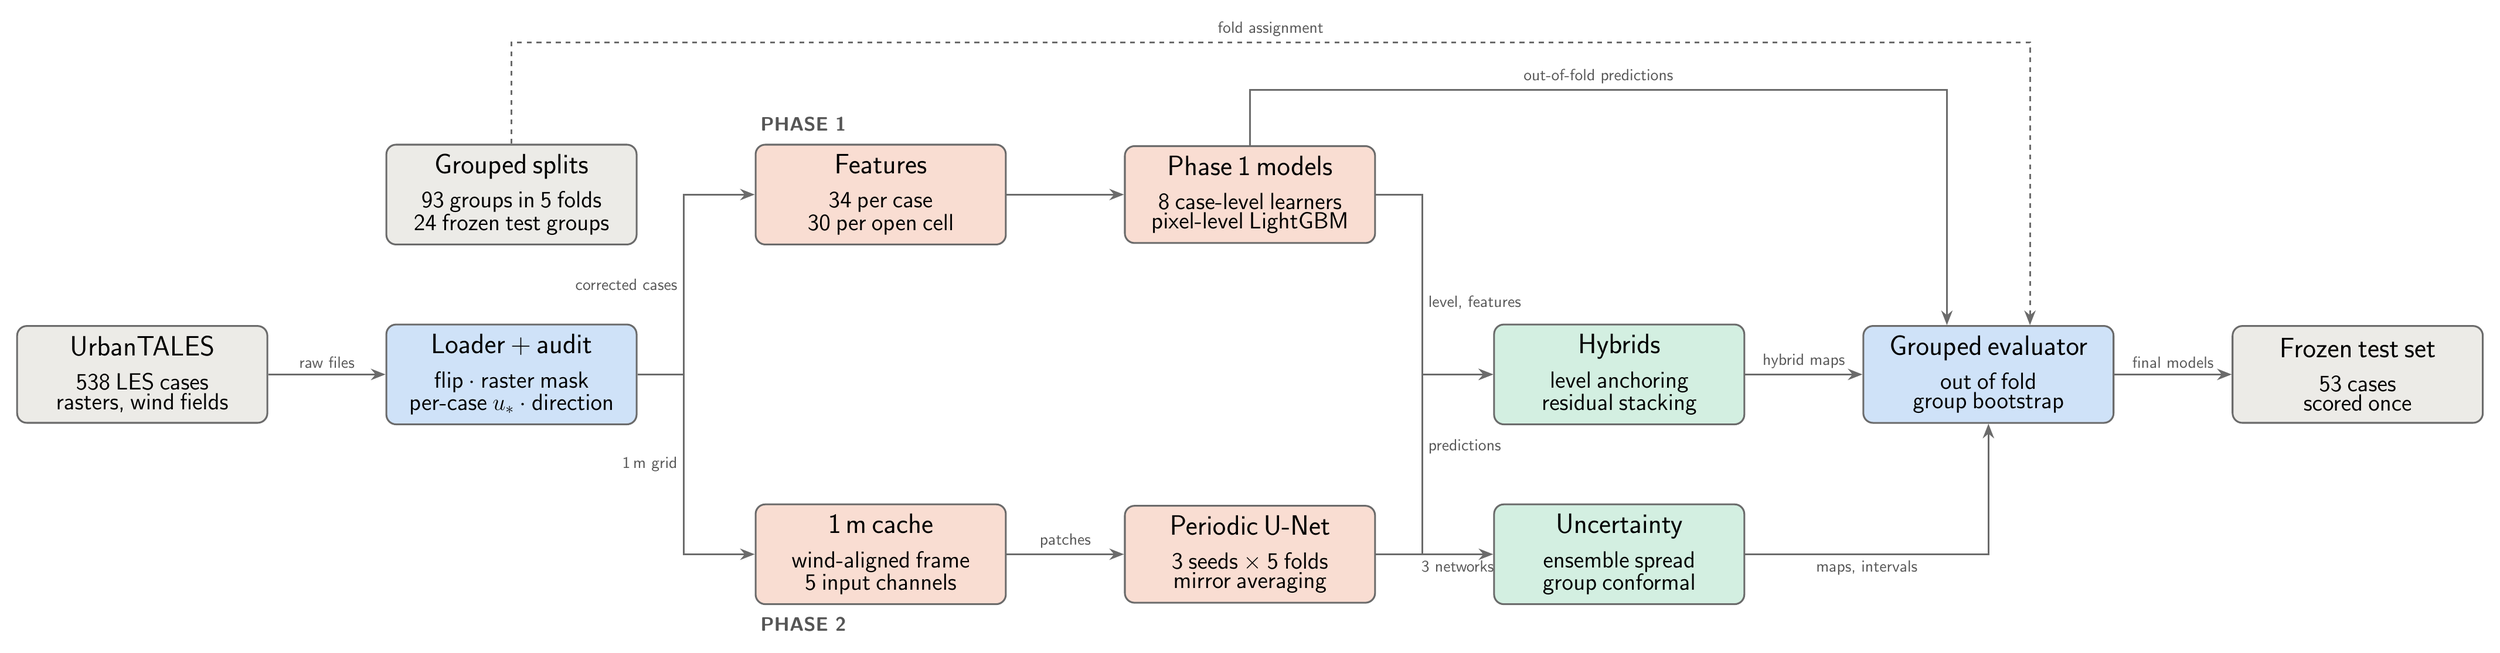
\begin{tikzpicture}
\def\dx{8.0}
\node[data] (ut) at (0,-4.8) {\nt{UrbanTALES}{538 LES cases\\rasters, wind fields}};
\node[ctrl] (ld) at (\dx,-4.8) {\nt{Loader + audit}{flip $\cdot$ raster mask\\per-case $u_*$ $\cdot$ direction}};
\node[data] (sp) at (\dx,-0.9) {\nt{Grouped splits}{93 groups in 5 folds\\24 frozen test groups}};
\node[path] (ft) at (2*\dx,-0.9) {\nt{Features}{34 per case\\30 per open cell}};
\node[path] (p1) at (3*\dx,-0.9) {\nt{Phase 1 models}{8 case-level learners\\pixel-level LightGBM}};
\node[path] (cc) at (2*\dx,-8.7) {\nt{1\,m cache}{wind-aligned frame\\5 input channels}};
\node[path] (un) at (3*\dx,-8.7) {\nt{Periodic U-Net}{3 seeds $\times$ 5 folds\\mirror averaging}};
\node[ana] (hy) at (4*\dx,-4.8) {\nt{Hybrids}{level anchoring\\residual stacking}};
\node[ana] (uq) at (4*\dx,-8.7) {\nt{Uncertainty}{ensemble spread\\group conformal}};
\node[ctrl] (ev) at (5*\dx,-4.8) {\nt{Grouped evaluator}{out of fold\\group bootstrap}};
\node[data] (ts) at (6*\dx,-4.8) {\nt{Frozen test set}{53 cases\\scored once}};
\node[lane, anchor=south west] at ($(ft.north west)+(0,0.15)$) {PHASE 1};
\node[lane, anchor=north west] at ($(cc.south west)+(0,-0.15)$) {PHASE 2};
\draw[wire] (ut) -- node[lab, above] {raw files} (ld);
\coordinate (j1) at ($(ld.east)+(1.0,0)$);
\draw[wire] (ld.east) -- (j1) |- node[lab, pos=0.25, left] {corrected cases} (ft.west);
\draw[wire] (j1) |- node[lab, pos=0.25, left] {1\,m grid} (cc.west);
\draw[wire] (ft) -- (p1);
\draw[wire] (cc) -- node[lab, above] {patches} (un);
\coordinate (j2) at ($(p1.east)+(1.0,0)$);
\coordinate (j3) at ($(un.east)+(1.0,0)$);
\draw[wire] (p1.east) -- (j2) |- node[lab, pos=0.3, right] {level, features} (hy.west);
\draw[wire] (un.east) -- (j3) |- node[lab, pos=0.3, right] {predictions} (hy.west);
\draw[wire] (j3) -- node[lab, below] {3 networks} (uq.west);
\draw[wire] (hy) -- node[lab, above] {hybrid maps} (ev);
\draw[wire] (p1.north) -- ++(0,1.2) -| node[lab, pos=0.25, above] {out-of-fold predictions} ($(ev.north)+(-0.9,0)$);
\draw[wire] (uq.east) -| node[lab, pos=0.25, below] {maps, intervals} (ev.south);
\draw[dwire] (sp.north) -- ++(0,2.2) -| node[lab, pos=0.25, above] {fold assignment} ($(ev.north)+(0.9,0)$);
\draw[wire] (ev) -- node[lab, above] {final models} (ts);
\end{tikzpicture}
\end{document}
